%!TEX program = xelatex
\documentclass[dvipsnames, svgnames,a4paper,11pt]{article}
% ----------------------------------------------------- 
%	加边框的命令
%	参考:https://tex.stackexchange.com/questions/531559/how-to-add-the-page-border-for-first-two-pages-in-latex
\usepackage{tikz}
\usetikzlibrary{calc}
\usepackage{eso-pic}
\AddToShipoutPictureBG{%
\begin{tikzpicture}[overlay,remember picture]
\draw[line width=0.6pt] % 边框粗细
    ($ (current page.north west) + (0.6cm,-0.6cm) $)
    rectangle
    ($ (current page.south east) + (-0.6cm,0.6cm) $); % 边框位置
\end{tikzpicture}}


\usepackage{xcolor}
\definecolor{c1}{HTML}{086173} % 目录颜色 原版为2752C9 紫灰色535AAA 蓝紫色0B0DB7 深蓝色070F94 湖绿色219394 松石灰绿086173
\definecolor{c2}{HTML}{E20129} % 引用颜色 原版\definecolor{c2}{RGB}{190,20,83} 橙色F24729

\usepackage{ctex}
\usepackage[top=28mm,bottom=28mm,left=15mm,right=15mm]{geometry}
\usepackage{hyperref} 
\hypersetup{
	colorlinks,
	linktoc = section, % 超链接位置,选项有section, page, all
	linkcolor = c1, % linkcolor 目录颜色
	citecolor = c1  % citecolor 引用颜色
}
\usepackage{amsmath,enumerate,multirow,float}
\usepackage{tabularx}
\usepackage{tabu}
\usepackage{subfig}
\usepackage{fancyhdr}
\usepackage{graphicx}
\usepackage{wrapfig}  
\usepackage{physics}
\usepackage{appendix}
\usepackage{amsfonts}

%
\usepackage{tcolorbox}
\tcbuselibrary{skins,breakable}
\newtcolorbox{tbox}[2][]{
    colframe=black!70!,
    breakable,
    enhanced,
	boxrule =0.5pt,
    title = {#2},
    fonttitle = \large\kaishu\bfseries,
	drop fuzzy shadow,
    #1
}
\newtcolorbox[auto counter,number within=section]{question}[1][]{
  top=2pt,bottom=2pt,arc=1mm,
  boxrule=0.5pt,
%   frame hidden,
  breakable,
  enhanced, %跨页后不会显示下边框
  coltitle=c1!80!gray,
  colframe=c1,
  colback=c1!3!white,
  drop fuzzy shadow,
  title={思考题~\thetcbcounter:\quad},
  fonttitle=\bfseries,
  attach title to upper,
  #1
}

% ---------------------------------------------------------------------
%	利用cleveref改变引用格式,\cref是引用命令
\usepackage{cleveref}
\crefformat{figure}{#2{\textcolor{c2}{Figure #1}}#3} % 图片的引用格式
\crefformat{equation}{#2{(\textcolor{c2}{#1})}#3} % 公式的引用格式
\crefformat{table}{#2{\textcolor{c2}{Table #1}}#3} % 表格的引用格式


% ---------------------------------------------------------------------
%	页眉页脚设置
\fancypagestyle{plain}{\pagestyle{fancy}}
\pagestyle{fancy}
\lhead{\kaishu 中山大学物理与天文学院电子技术实验\uppercase\expandafter{\romannumeral1}} % 左边页眉,学院 + 课程
\rhead{\kaishu 实验报告By黄罗琳} % 右边页眉,实验报告标题
\cfoot{\thepage} % 页脚,中间添加页码


% ---------------------------------------------------------------------
%	对目录、章节标题的设置
\renewcommand{\contentsname}{\centerline{\huge 目录}}
\usepackage{titlesec}
\usepackage{titletoc}
% \titleformat{章节}[形状]{格式}{标题序号}{序号与标题间距}{标题前命令}[标题后命令]
\titleformat{\section}{\centering\LARGE\songti}{}{1em}{}

% ---------------------------------------------------------------------
%   listing代码环境设置
\usepackage{listings}
\lstloadlanguages{python}
\lstdefinestyle{pythonstyle}{
backgroundcolor=\color{gray!5},
language=python,
frameround=tftt,
frame=shadowbox, 
keepspaces=true,
breaklines,
columns=spaceflexible,                   
basicstyle=\ttfamily\small, % 基本文本设置,字体为teletype,大小为scriptsize
keywordstyle=[1]\color{c1}\bfseries, 
keywordstyle=[2]\color{Red!70!black},   
stringstyle=\color{Purple},       
showstringspaces=false,
commentstyle=\ttfamily\scriptsize\color{green!40!black},%注释文本设置,字体为sf,大小为smaller
tabsize=2,
morekeywords={as},
morekeywords=[2]{np, plt, sp},
numbers=left, % 代码行数
numberstyle=\it\tiny\color{gray}, % 代码行数的数字字体设置
stepnumber=1,
rulesepcolor=\color{gray!30!white}
}




% ---------------------------------------------------------------------
%	其他设置
\def\degree{${}^{\circ}$} % 角度
\graphicspath{{./images/}} % 插入图片的相对路径
\allowdisplaybreaks[4]  %允许公式跨页 
\usepackage{lipsum}
\usepackage{adjustbox}
%\usepackage{mathrsfs} % 字体
%\captionsetup[figure]{name=Figure} % 图片形式
%\captionsetup[table]{name=Table} % 表格形式
\begin{document}
	
	% 实验报告封面	
	% 顶栏
	\begin{table}
		\renewcommand\arraystretch{1.7}
		\begin{tabularx}{\textwidth}{
				|X|X|X|X
				|X|X|X|X|}
			\hline
			\multicolumn{2}{|c|}{预习报告}&\multicolumn{2}{|c|}{实验记录}&\multicolumn{2}{|c|}{分析讨论}&\multicolumn{2}{|c|}{总成绩}\\
			\hline
			\LARGE25 & & \LARGE25 & & \LARGE30 & & \LARGE80 & \\
			\hline
		\end{tabularx}
	\end{table}
	% ---
	
	% 信息栏
		\begin{table}
		\renewcommand\arraystretch{1.7}
		\begin{tabularx}{\textwidth}{|X|X|X|X|}
			\hline
			年级、专业: & 2022级 物理学 &组号: &D8 \\
			\hline
			姓名: &  黄罗琳,王显  & 学号: &22344001 22344002   \\
			\hline
			实验时间: & 2024/3/20 & 教师签名: & \\
			\hline
		\end{tabularx}
	\end{table}
	% ---
	
	% 大标题
	\begin{center}
	\LARGE ET4 \quad 戴维南定理和诺顿定理
	\end{center}
	% ---
	
	% 注意事项
	
	% 基本
	\textbf{【实验报告注意事项】}
	\begin{enumerate}
		\item 实验报告由三部分组成:
		\begin{enumerate}
			\item 预习报告:课前认真研读实验讲义,弄清实验原理;实验所需的仪器设备、用具及其使用、完成课前预习思考题;了解实验需要测量的物理量,并根据要求提前准备实验记录表格(可以参考实验报告模板,可以打印)。\textcolor{red}{\textbf{(20分)}}
			\item 实验记录:认真、客观记录实验条件、实验过程中的现象以及数据。实验记录请用珠笔或者钢笔书写并签名(\textcolor{red}{\textbf{用铅笔记录的被认为无效}})。\textcolor{red}{\textbf{保持原始记录,包括写错删除部分,如因误记需要修改记录,必须按规范修改。}}(不得输入电脑打印,但可扫描手记后打印扫描件);离开前请实验教师检查记录并签名。\textcolor{red}{\textbf{(30分)}}
			\item 数据处理及分析讨论:处理实验原始数据(学习仪器使用类型的实验除外),对数据的可靠性和合理性进行分析;按规范呈现数据和结果(图、表),包括数据、图表按顺序编号及其引用;分析物理现象(含回答实验思考题,写出问题思考过程,必要时按规范引用数据);最后得出结论。\textcolor{red}{\textbf{(30分)}}
		\end{enumerate}
		\textbf{实验报告就是将预习报告、实验记录、和数据处理与分析合起来,加上本页封面。\textcolor{red}{(80分)}}
		\item 实验报告在\textcolor{red}{\textbf{每个小结(补做)的之后一周内}}提交,最后一次实验,在\textcolor{red}{\textbf{结束一周内}}提交。
		
	\end{enumerate}
	

	% 目录
	\clearpage
	\tableofcontents
	\clearpage
	% ---
	
	
	
	% 预习报告	
	
	% 小标题
	\setcounter{section}{0}
\section{ET4戴维南定理和诺顿定理 \quad\heiti 预习报告}
	% ---
	
	% 实验目的
	\subsection{实验目的}
	\begin{enumerate}
		\item 加深对戴维南定理和诺顿定理的理解。
	\item 学习戴维南等效参数的各种测量方法。
	\item 理解等效置换的概念。
	\item 学习直流稳压电源、万用表、直流电流表和电压表的正确使用方法。
	\end{enumerate}
	% ---
	
	% 仪器用具
	\subsection{仪器用具}
	\begin{table}[htbp]
		\centering
		\renewcommand\arraystretch{1.6}
		% \setlength{\tabcolsep}{10mm}
		\begin{tabular}{|p{0.05\textwidth}|p{0.20\textwidth}|p{0.05\textwidth}|p{0.5\textwidth}|}
			\hline
			编号& 仪器用具名称 & 数量 &  主要参数(型号,测量范围,测量精度等) \\
			\hline
			1& 电路原理箱或板 & 1 & 戴维南定理和诺顿定理 \\
			\hline
			2& 稳压源 & 1 &  RIGOL DP831\\
			\hline
			3& 直流电流源 & 1 &  \\
			\hline
			4& 直流电流表 & 3 & RIGOL DM3058E \\
			\hline
			5& 直流电压表 & 2 &  RIGOL DM3058E\\
			\hline
			6& 电流表专用线 & 3 &  \\
			\hline
			7& 2号实验导线 & n &  \\
			\hline
			8& 其它 & -- &  \\
			\hline
		\end{tabular}
	\end{table}
	% ---
	
	% 原理概述
	\subsection{原理概述}
	\begin{enumerate}
	\item \textbf{戴维南定理}指出:对于一个含有独立电源、线性电阻和受控源的一端口,可以用一个电压源和电阻的串联组合来等效置换。其中,该电压源的激励电压等于端口的开路电压,电阻等于将端口内全部独立电源置零后的输入电阻。
	\item \textbf{诺顿定理}是戴维南定理的对偶形式。它指出:对于一个含有独立电源、线性电阻和受控源的一端口,可以用一个电流源和电阻的并联组合来等效置换。电流源的激励电流等于端口的短路电流,电阻等于将端口中全部独立源置零后的输入电阻。
	\item \textbf{戴维南-诺顿定理的等效电路}是对外部特性而言的。换句话说,无论网络内部是时变的还是定常的,只要网络内部除了独立电源外都是线性元件,上述等效电路都是正确的。测量戴维南等效电路参数的方法:对于开路电压 $U_{oc}$ 的测量,可以直接使用电压表测量,也可以采用补偿法测量;而对于戴维南等效电阻 $R_{eq}$ 的获取,可采用如下方法:当网络含有源时,可以使用开路电压法或者短路电流法,但对于不允许直接短路外部电路的网络(例如,可能因短路电流过大而损坏网络内部器件的情况),不能采用短路电流法;当网络不含源时,可以使用伏安法、半流法、半压法、直接测量法等方法。
\end{enumerate}
\begin{figure}[H]
	\centering
	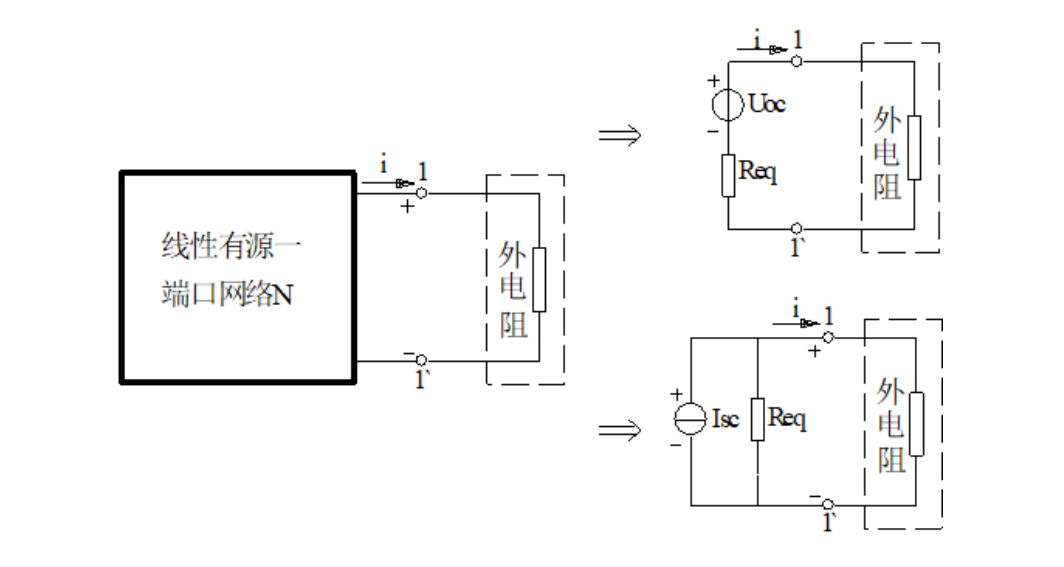
\includegraphics[width=0.4\linewidth]{images/一种端口}
	\caption{一种端口网络的等效置换}
	\label{fig:}
\end{figure}
	% ---
	
	
	
	% 实验前思考题
	\subsection{实验预习题}
	
\begin{question}
	用开路电压、短路电流法测量等效电阻时,开路电压、短路电流是否可以同时进行测量,为什么?
\end{question}

在使用开路电压和短路电流法测量电路的等效电阻时,实际操作中开路电压和短路电流是不能同时进行测量的。原因在于这两种测量方式的条件和对电路的影响完全不同。

\textbf{开路电压测量}:在进行开路电压的测量时,测量对象的两端不接任何外部负载,即电路是开路状态。这种测量方式的目的是测定在无负载条件下电源的电压,即电源的最大电动势。在这种状态下,电路中的电流为零,因此不会有电流通过被测电源或电路,可以获得一个准确的开路电压值。

\textbf{短路电流测量}:而在进行短路电流的测量时,测量对象的两端被直接短路,通过一个极低的电阻(接近于零),目的是测量在这种极端条件下通过电路的电流大小。这种状态下电路的电阻最小,电流达到最大值。这样做可以确定电源或电路在最大负载条件下的输出电流能力。

由于开路状态下电路的电流为零,而短路状态下电流达到最大,这两种状态下的电路条件截然不同,因此不能同时进行测量。同时,若尝试同时进行这两种测量,可能会导致测量结果不准确,甚至损坏测量设备或被测电路。通常,在实际应用中,先后分别进行这两种测量,然后通过欧姆定律(V=IR)计算出等效电阻值,即使用开路电压除以短路电流的方法得到等效电阻值:$ R_{\text{等效}} = \dfrac{V_{\text{开路}}}{I_{\text{短路}}} $。
	
	
	% 实验记录	
	\clearpage
	
	% 顶栏
	\begin{table}
		\renewcommand\arraystretch{1.7}
		\centering
		\begin{tabularx}{\textwidth}{|X|X|X|X|}
			\hline
			专业: & 物理学 & 年级: & 2022级 \\
			\hline
			姓名: & 黄罗琳,王显& 学号: &22344001,22344002 \\
			\hline
			室温: &  25℃& 实验地点: & A522 \\
			\hline
			学生签名:& 
\includegraphics[width=1cm]{签字.jpg} 
\includegraphics[width=1cm]{wx.jpg}  & 评分: &\\
			\hline
			实验时间:& 2024/3/20 & 教师签名:&\\
			\hline
		\end{tabularx}
	\end{table}
	% ---
	
	% 小标题
	\section{ET4戴维南定理和诺顿定理  \quad\heiti 实验记录}
	% ---
	
	% 实验过程记录
	\subsection{实验内容、步骤与结果}
	
	%
	\subsubsection{测量开路电压,短路电流} 
	设定Usn=12V
	\begin{enumerate}
		\item
		直接测量法
		 \begin{figure}[H]
			\centering
			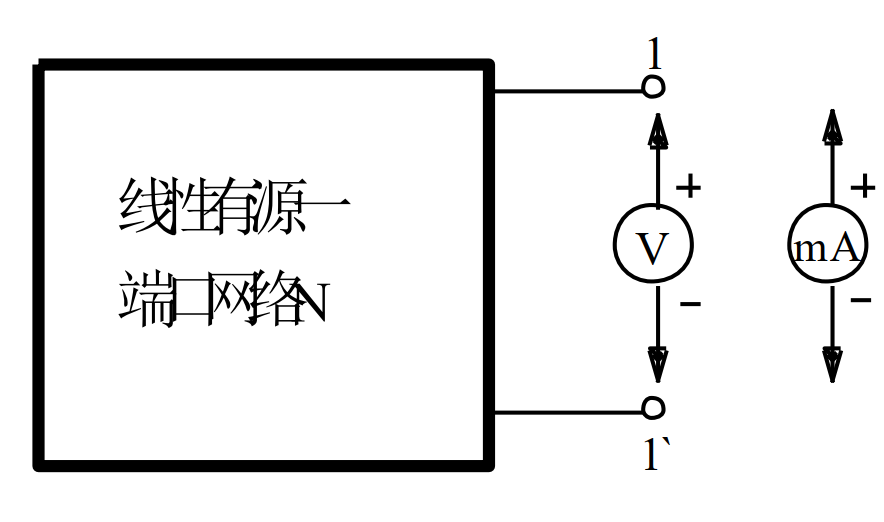
\includegraphics[width=0.4\linewidth]{开路电压.png}
			\caption{开路电压、短路电路法电路图}
			\label{}
		  \end{figure}
		 $\mathrm{U=3.93V~,~I=19.609mA}$
		  \item 间接测量法(补偿法)
		 \begin{figure}[H]
			\centering
			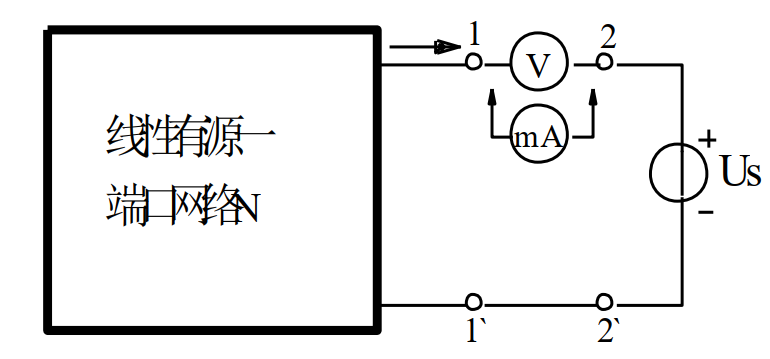
\includegraphics[width=0.4\linewidth]{电压零.png}
			\caption{间接测量法电路图}
			\label{}
		 \end{figure}
		 \begin{enumerate}
	     
		 \item 电压零示法\\
		 最初设定外加电压为 3.9V、0.1A  ,在直接测量法中结果为3.93V,故选3.9V为初始电压设定 \\电压(电压表零示数结果):2.665mV \\
		 最终调节外加电压为$\text{U=3.93V}$
		 
		 \item 电路零示法\\
		  最初设定外加电压为 3.9V、0.1A,选定3.93V原因与电压零示法相同  \\ 电流(电流表零示数结果):0.112mA\\
		 最终调节外加电压为$\text{U=3.93V}$
		 
		 \end{enumerate}	
		 
		 
	    
		
	\end{enumerate}	
	\subsubsection{测量等效电阻} 
	\begin{enumerate}

     \item 开路电压、短路电流法(内部有源)\\
	 $U=U_{oc}=3.93V,I=I_{sc}=19.609mA$,$R_{\mathrm{eq}}=200. 41817 \Omega $
	 \item 伏安法(内部无源)
	     \begin{figure}[{H}]
			\centering
			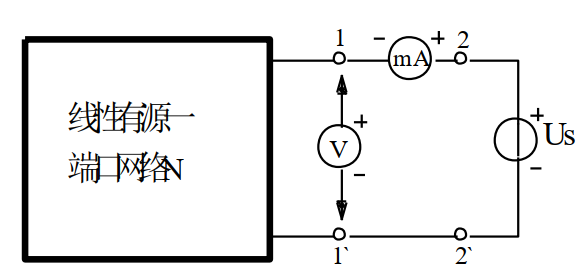
\includegraphics[width=0.6\linewidth]{伏安法电路图.png}
			\caption{伏安法电路图}
			\label{}
		 \end{figure}
		 \begin{table}[h]
			\centering
			\begin{tabular}{|c|c|c|}
			\hline
			$U_s$ (V) & $I_s$ (mA) & $U_v$ (V) \\
			\hline
			1 & 4.997 & 0.993 \\
			2 & 9.954 & 1.985 \\
			3 & 14.839 & 2.963 \\
			4 & 19.795 & 3.952 \\
			5 & 24.747 & 4.940 \\
			6 & 29.704 & 5.928 \\
			7 & 34.667 & 6.916 \\
			8 & 39.634 & 7.905 \\
			9 & 44.747 & 8.925 \\
			10 & 49.755 & 9.918 \\
			\hline
			\end{tabular}
			\caption{伏安法实验数据}
			\label{tab:data}
			\end{table}
			\item 半流法(内部无源)
			\begin{figure}[{H}]
				\centering
				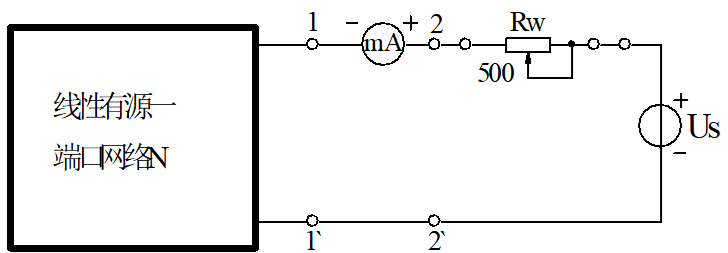
\includegraphics[width=0.4\linewidth]{半流法.png}
				\caption{半流法电路图}
				\label{}
			\end{figure}
			使用伏安法中$U_s=10V$时电流为$49.755mA$\\目标电流为$24.8775mA$\\
			最终测得$R_w=R_{\mathrm{eq}}=196.341 \Omega $
			\item 半压法(内部无源)
			\begin{figure}[{H}]
				\centering
				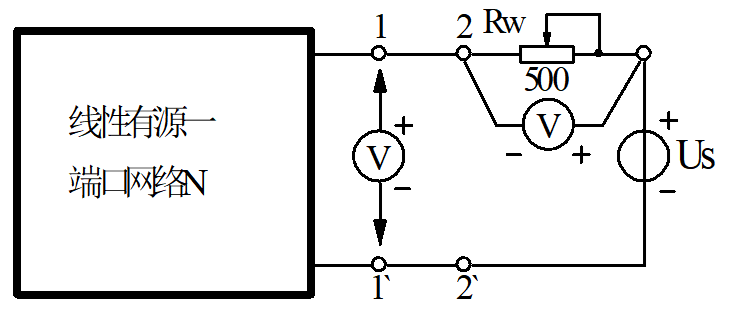
\includegraphics[width=0.4\linewidth]{半压法.png}
				\caption{半压法电路图}
				\label{}
			\end{figure}
			设定$U_s=10V$,调整到$U_{Rw}=5.051V$\\
			最终测得$R_w=196.941\Omega$
			

		 
	\end{enumerate}
	\subsubsection{验证戴维南定理} 
\begin{figure}[{H}]
	\centering
	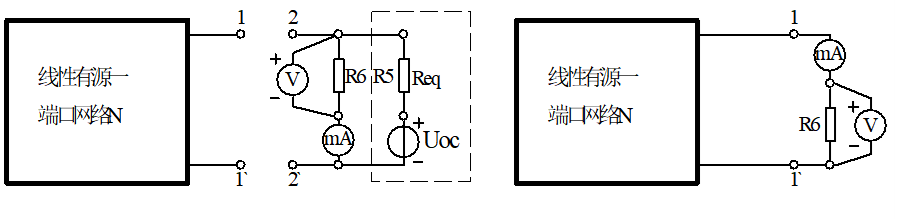
\includegraphics[width=0.9\linewidth]{戴维南定理.png}
	\caption{戴维南定理电路图}
	\label{}
\end{figure}
使用$U_{oc}$进行测量,并且等效电阻$R_5=R_{eq}=200\Omega$,外接$R_6=100\Omega$
 测得$U=1.304V $   $I=13.074mA$\\
 \indent 使用N有源网络端口外接负载$R_6=100\Omega$
 测得$U=1.3077V$   $ I=13.119mA$
 \subsubsection{验证诺顿定理}
 \begin{figure}[{H}]
	\centering
	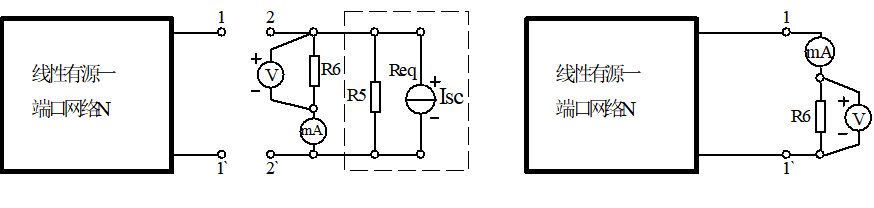
\includegraphics[width=0.9\linewidth]{诺顿定理.png}
	\caption{诺顿定理实验电路图}
	\label{}
 \end{figure}
 使用$I_{sc}$进行测量,并且将戴维南等效电阻$R_5=R_{eq}=200\Omega$并联后,外接$R_6=100\Omega$。\\
\indent 测得$U=1.30418V$   $ I=13.016mA$
\subsubsection{测量实验室函数信号发生器的戴维南等效内阻}
 实验电路图采用半压法电路图
 \begin{figure}[{H}]
	\centering
	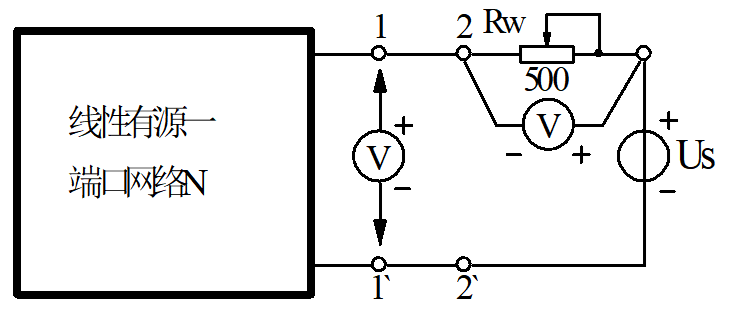
\includegraphics[width=0.6\linewidth]{半压法.png}
	\caption{实验电路图(左侧连接信号发生器)}
	\label{}
 \end{figure}
 初始值设定信号发生器为:$f = 1\, \text{kHz} \quad V_{\text{pp}} = 2500\, \text{mV} $\\
 \indent $\text{使用半压法:} \quad U_s = 6\, \text{V} $\\
 \indent $50\Omega \quad U = 3.015\, \text{V} \quad R_w = 51.7942\, \Omega $\\
 \indent 高阻$ U = 2.997\, \text{V} \quad R_w = 52.665\, \Omega$\\
 \indent 初始值设定信号发生器为:$f = 1\, \text{kHz} \quad V_{\text{pp}} = 2500\, \text{mV} $\\
 \indent $\text{使用半压法:} \quad U_s = 8\, \text{V} $\\
 \indent $50\Omega \quad U = 4.000\, \text{V} \quad R_w = 52.501\, \Omega $\\
 \indent 高阻$ U = 4.041\, \text{V} \quad R_w = 52.638\, \Omega$

 根据实验结果分析:负载不同时,Rw变化很小.负载 $50\Omega$ 的信号是高负载的两倍
 
	
	% 原始数据
	\clearpage
	
	% ---
	
	% 问题记录
	\subsection{实验过程遇到问题及解决办法}
	\begin{enumerate}
		\item 实验过程中接线需要仔细思考,有些接线并不能很好的满足仪器的接口要求,就需要寻找符合要求的线材进行接线,从而完成实验电路图。
		\item 在测量电流时,台式万用表的读数会在一定范围内进行变化,这可能是由于电流流过导致温度升高从而出现了阻值变化,所以在实验过程中统一选取电流稳定时的某一示数,保证了误差在一定范围内。
		\item 在进行\textbf{测量实验室函数信号发生器的戴维南等效内阻}这一实验中时,起初对实验电路的内部构造不够了解,最后通过老师的讲解理解了为什么负载不同信号会出现变化。
	\end{enumerate}
	% ---
	
	
	
	% 分析与讨论	
	\clearpage
	
	% 顶栏
	\begin{table}
		\renewcommand\arraystretch{1.7}
		\begin{tabularx}{\textwidth}{|X|X|X|X|}
			\hline
			专业:& 物理学 &年级:& 2022级\\
			\hline
			姓名: & 黄罗琳、王显 & 学号:&22344001 22344002 \\
			\hline
			日期:& 2024/3/20 & 评分: &\\
			\hline
		\end{tabularx}
	\end{table}
	% ---
	
	% 小标题
	\section{ET4戴维南定理和诺顿定理\quad\heiti 分析与讨论}
	% ---
	
	% 数据处理
	\subsection{对于有源一端口的理论计算}
	\begin{figure}[H]
		\begin{minipage}[b]{0.45\linewidth}
			\centering
			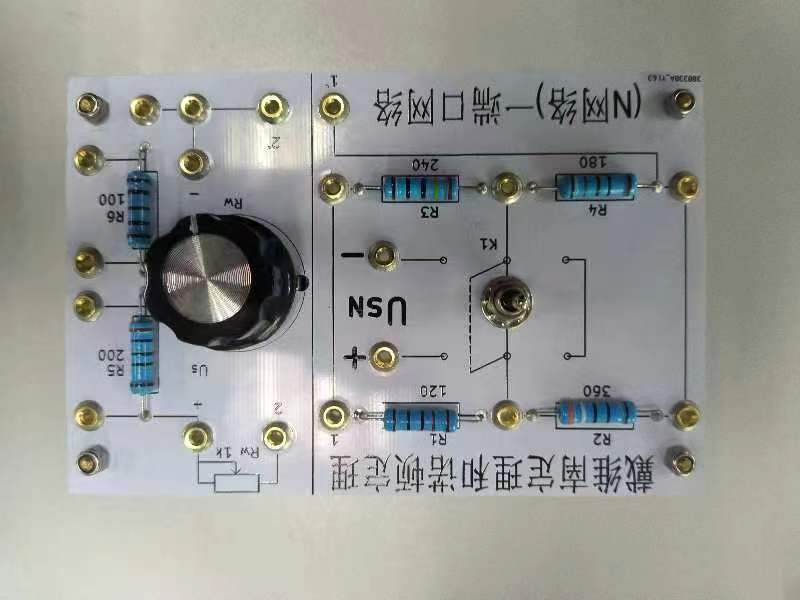
\includegraphics[width=\linewidth]{原始电路板.jpg}
			\caption{实验所用电路板}
		\end{minipage}
		\hfill
		\begin{minipage}[b]{0.45\linewidth}
			\centering
			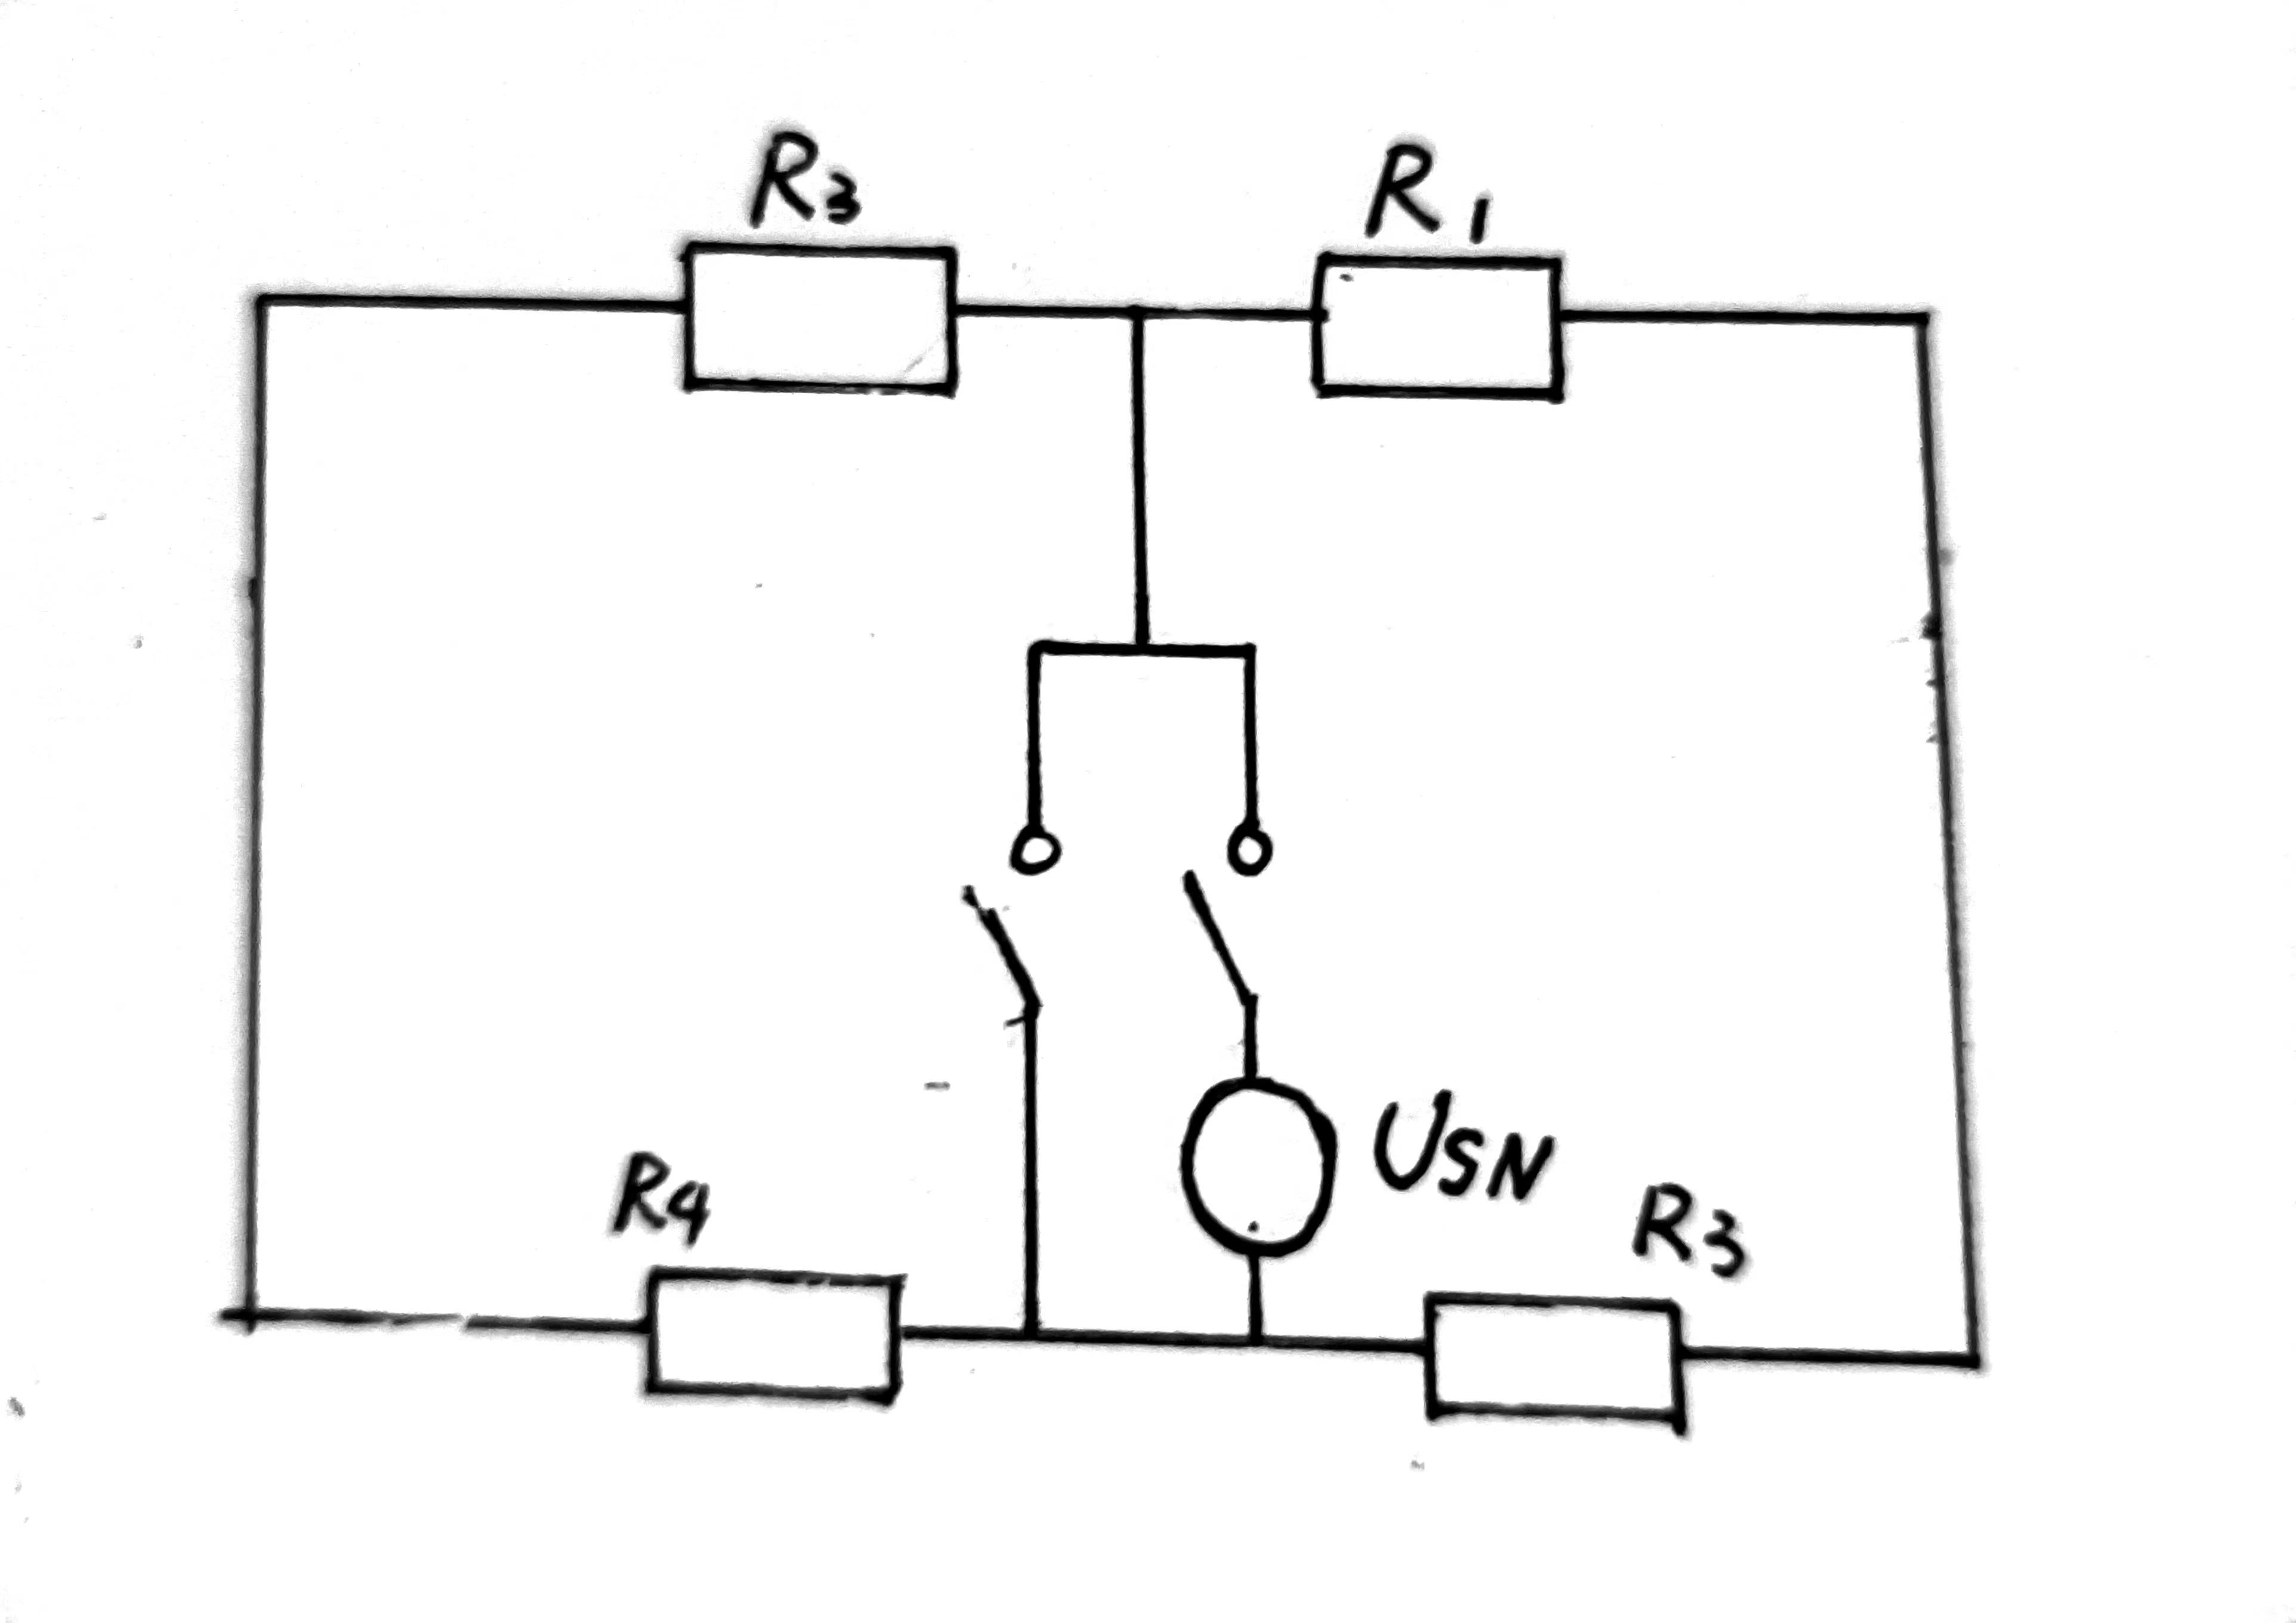
\includegraphics[width=\linewidth]{手绘.jpg}
			\caption{使用N有源网络内部电路图}
		\end{minipage}
	\end{figure}
	计算可得其内部电阻理论值为$R=200 \Omega $,基于此项数据对实验结果进行如下误差分析。
	\subsection{测量开路电压、短路电流}
	
	%
	\subsubsection{直接测量法测量}
	$\mathrm{U=3.93V~,~I=19.609mA}$\\
	\indent 而理论值$\mathrm{U=4V~,~I=20mA}$\\
	\indent 则相对误差为:$r=-1.75\%$\quad$r=-1.99\%$ \\
	\indent 误差可能来源于:N网络内部的电阻与设定阻值不同,可能更大,从而导致了,内阻增大,从而导致了分压增大,从而电压变小,短路电流减少。
	\subsubsection{间接测量法(电路图)}
	\begin{enumerate}
		\item 电压零示法\\
		测量值:$\text{U=3.93V}$\quad 电压(电压表零示数结果):2.665mV \\
		理论值为:$\text{U=4V}$
		\quad 相对误差为:$r=-1.75\%$\\
		误差可能来源于:除与直接测量法相同的误差来源之外(内阻更大),还可能是因为在实验过程调整电压表为零时,仅仅是调整电压为2.665mV,从而导致测量值比实际值较小,但是虽然出现不为零的情况。\textbf{但是其测量值仍在3.93V附近,所以说明误差仍是内阻导致的问题。}
		\item 电流零示法\\
		测量值:$\text{U=3.93V}$\quad 电流(电流表零示数结果):0.112mA \\
		理论值为:$\text{U=4V}$
		\quad 相对误差为:$r=-1.75\%$\\
		误差可能来源于:电流表不能完全到达零示数,但是其仍然在3.93V附近。并且由于仪器精度问题,其与电压零示法结果相同,均为3.93V。
	\end{enumerate}
	
	%
	\subsection{测量等效电阻}
	
		\subsubsection{开路电压、短路电流法}
	 $U=U_{oc}=3.93V,I=I_{sc}=19.609mA$,$R_{\mathrm{eq}}=200. 41817 \Omega $\\
	 \indent 与理论值$R=200 \Omega $比较,相对误差为:$r=0.209\%$\\\indent 
	 误差可能来源于电流表的内阻引入的,与电路串联后导致所测量的电阻增大。
	 \subsubsection{伏安法} 
	  根据实验数据进行图像拟合,如下所示:
	  \begin{figure}[{H}]
		\centering
		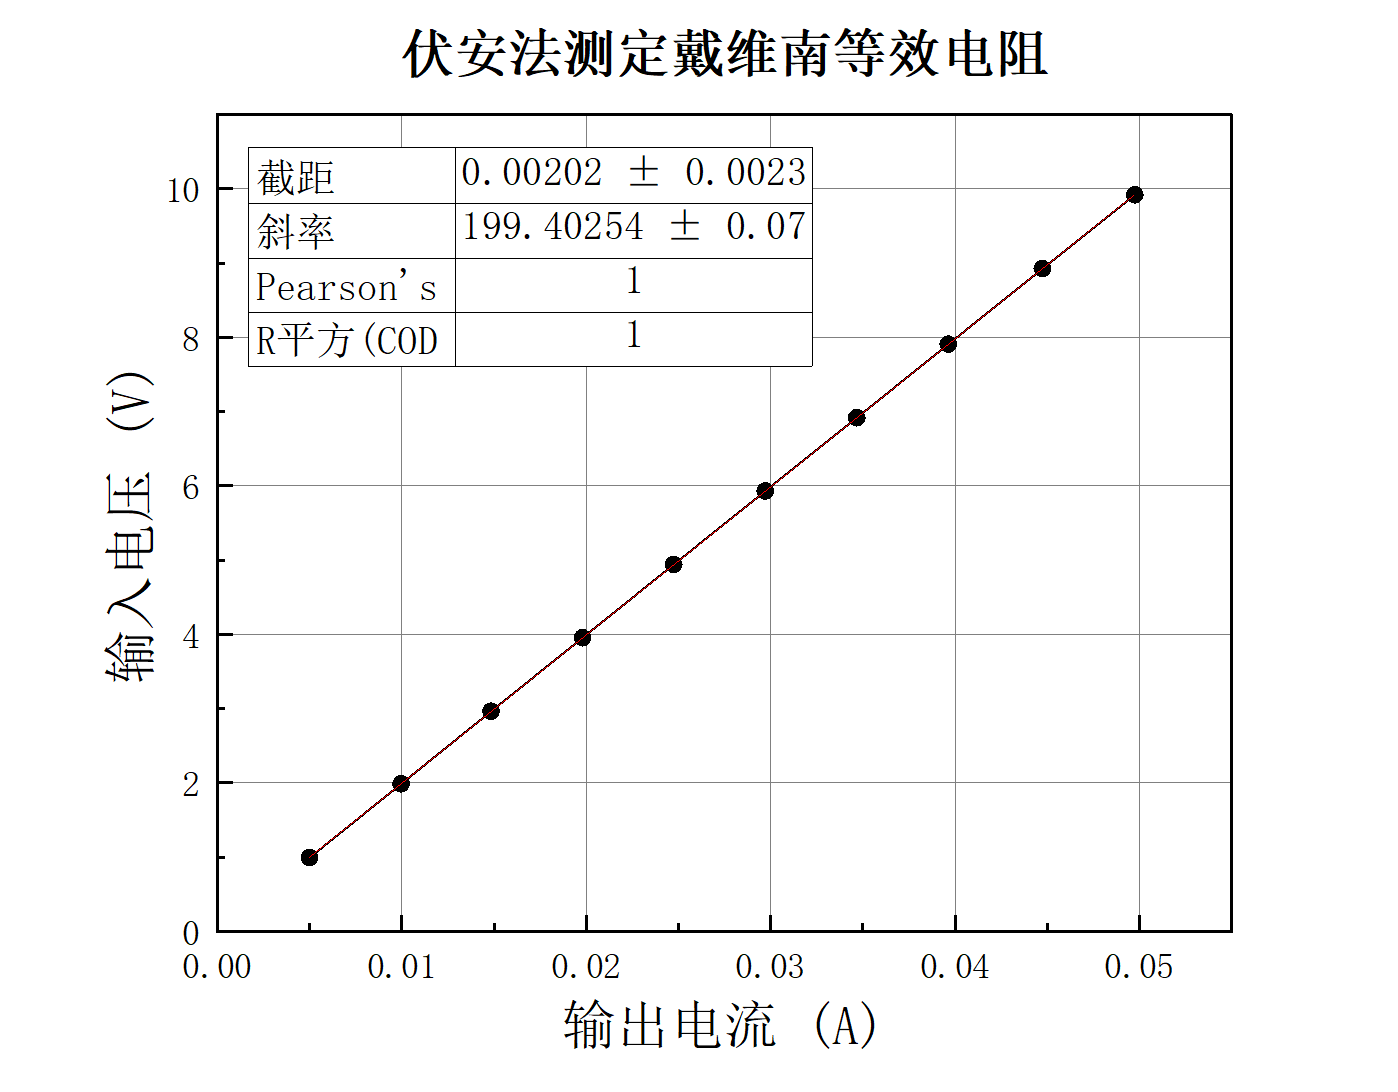
\includegraphics[width=0.6\linewidth]{拟合.png}
		\caption{伏安法拟合图像}
		\label{}
	  \end{figure}
	  根据图像斜率可知:$R_{\mathrm{eq}}=199.40254\Omega $
	  \\ \indent 与理论值$R=200 \Omega $比较,相对误差为:$r=-0.299\%$\\
	  \indent 实验误差相比于其他实验方法明显偏小,这说明通过线性拟合的方式可以得到更加准确的结果。
	  \subsubsection{半流法}
	  测得$R_w=R_{\mathrm{eq}}=196.341 \Omega $
\\ \indent 与理论值$R=200 \Omega $比较,相对误差为:$r=-1.830\%$\\
\indent 误差可能来源于电表的示数存在一定的精度问题,\textbf{不能做到完全的精确一半的电流},从而计算结果与实际存在较小的差距。并且可能由于调整目标电流时电流值存在一定的波动,导致最终实验结果存在误差,并且在测量阻值时也会存在仪器误差,并且变阻器的调整会出现主观的操作问题(难以准确控制)并且接入电路的电源也可能存在内阻,这也会导致实验出现误差。\\
\indent 这些误差影响综合起来,导致了实验结果比理论值偏小。
\subsubsection{半压法} 
 测得$R_w=R_{\mathrm{eq}}=196.941 \Omega $
 \\\indent 与理论值$R=200 \Omega $比较,相对误差为:$r=-1.530\%$\\
 \indent 误差来源基本上与半流法误差来源相同,电表的示数存在一定的精度问题,\textbf{不能做到完全的精确一半的电压}。\\

	% ---
	
	% 实验后思考题
	\subsection{验证戴维南定理}
	使用等效电路测得$U=1.304V $   $I=13.074mA$\\
	\indent 使用N有源网络端口测得$U=1.3077V$   $ I=13.119mA$\\
	\indent 计算电压的相对误差$r=-0.28\%$ 电流的相对误差$r=0.34\%$\\
    \indent \textbf{\Large{故可以验证戴维南定理成立!}}
	\subsection{验证诺顿定理}
	\indent 测得$U=1.30418V$   $ I=13.016mA$\\
	\indent 使用N有源网络端口测得$U=1.3077V$   $ I=13.119mA$\\
	\indent 计算电压的相对误差$r=0.27\%$ 电流的相对误差$r=0.79\%$\\
	\indent \textbf{\Large{故可以验证诺顿定理成立!}}
	\subsection{测量实验室函数信号发生器的戴维南等效内阻}
	\indent 负载为$50\Omega 时\quad U = 4.000\, \text{V} \quad R_w = 52.501\, \Omega $\\
 \indent 负载为高阻时$ U = 4.041\, \text{V} 时\quad R_w = 52.638\, \Omega$\\
 \indent \textbf{负载不同时,Rw变化很小.负载 $50\Omega$ 的信号是高负载的两倍}\\
 \indent \textbf{函数信号发生器的等效内阻是一个重要的参数,它描述了信号发生器在连接到外部负载时所表现出的电阻性质。该参数与信号发生器的内部结构密切相关,包括波形发生电路和输出电路。在连接外部负载时,外部负载与信号发生器的等效内阻构成一个电路,这个电路的特性受到外部负载阻抗的影响,包括输出电压和输出功率的稳定性。一些函数信号发生器具有高阻特性,能够在连接到高阻负载时提供相对稳定的输出信号,不会因负载变化而产生明显的失真或输出电压的变化。}

\subsection{误差分析综述}
\begin{table}[htbp]
	\centering
	\begin{tabular}{|c|c|c|c|c|}
		\hline
		& 理论计算 & 直接测量   & 电压零示法 & 电流零示法 \\
		\hline
		$U_{OC}/V$ & 4.000    & 3.93 & 3.93 & 3.93 \\
		\hline
		相对误差  &    /  & -1.75\% & -1.75\%&-1.75\% \\
		\hline
	\end{tabular}
	\caption{测量有源一端口网络开路电压实验数据}
\end{table}


\begin{table}[H]
	\centering
	\begin{tabular}{|c|c|c|c|c|c|}
		\hline
		 & 理论计算 & 开路电压、短路电流法 & 伏安法 & 半流法 & 半压法 \\
		\hline
		 $R_{eq}/\Omega$  & 200  & 200.418     & 199.402& 196.341   & 196.941    \\
		 \hline
		相对误差 & / & 0.209\% & $-0.299\%$  & $-1.830\%$ & $-1.530\%$  \\
		\hline
	\end{tabular}
	\caption{测量有源一端口网络等效电阻实验数据}
\end{table}
\quad \\
\quad \\
概括上述误差分析和综合对比各个实验的相对误差,可以看出:
\begin{itemize}
    \item \textbf{直接测量法与间接测量法比较}:
    \begin{itemize}
        \item 直接测量法的相对误差为$-1.75\%$。主要误差可能来自于网络内部电阻与设定阻值不同,导致内阻增大,从而引起电压减小、短路电流减少。
        \item 间接测量法中,电压零示法和电流零示法的相对误差均为 $-1.75\%$。可能误差来源包括电压表、电流表的调零及内阻增大,但测量值仍在附近,表明误差主要由内阻引起。
    \end{itemize}
    \item \textbf{测量等效电阻的不同方法比较}:
    \begin{itemize}
        \item 开路电压、短路电流法得到的相对误差为 $0.209\%$。可能误差来自电流表的内阻导致电路总电阻增大。
        \item 伏安法得到的相对误差为 $-0.299\%$。误差相比其他方法明显偏小,说明通过线性拟合的方式得到了较为准确的结果。
        \item 半流法和半压法的相对误差分别为 $-1.830\%$ 和 $-1.530\%$。可能误差来源包括电表示数精度问题、目标电流或电压的波动、仪器误差以及主观操作引入的误差。
    \end{itemize}
    
\end{itemize}


	\clearpage

	\section{ET4戴维南定理和诺顿定理\quad\heiti 结语}
	% ---
	
	
	\subsection{实验心得和体会、意见建议等}
	\begin{enumerate}
		\item 实验总体过程属于思路非常清晰,从一开始测量简单的开路电压短路电流测量到最后验证两个定理,体现了由浅入深的难度和实验思路,实验过程中体验很好。
		\item 实验过程中会出现一些接线问题,通过对于实验仪器的逐渐熟悉,现在已经能够快速地找到适合本次实验仪器接口的接线,于是能够很快的完成实验。
		\item 实验的误差分析相对来说属于对于同样的误差进行分析,相关讨论见误差分析部分,这说明可能是由于实验教学电路板的仪器误差导致的,所以实验总体误差来说似乎来源于同样的问题。
		\item \textbf{本实验报告采用LATEX编辑,实验分工为黄罗琳同学负责记录数据、编辑报告、误差分析,王显同学负责实验操作、误差分析、数据绘图。}
	\end{enumerate}
	\quad \large \textbf{感谢您对于此篇实验报告的阅读与批改,祝您工作顺利!}
	% ---
	

	% 附件
	\subsection{附件}
	
	\begin{figure}[H]
		\begin{minipage}[b]{0.45\linewidth}
			\centering
			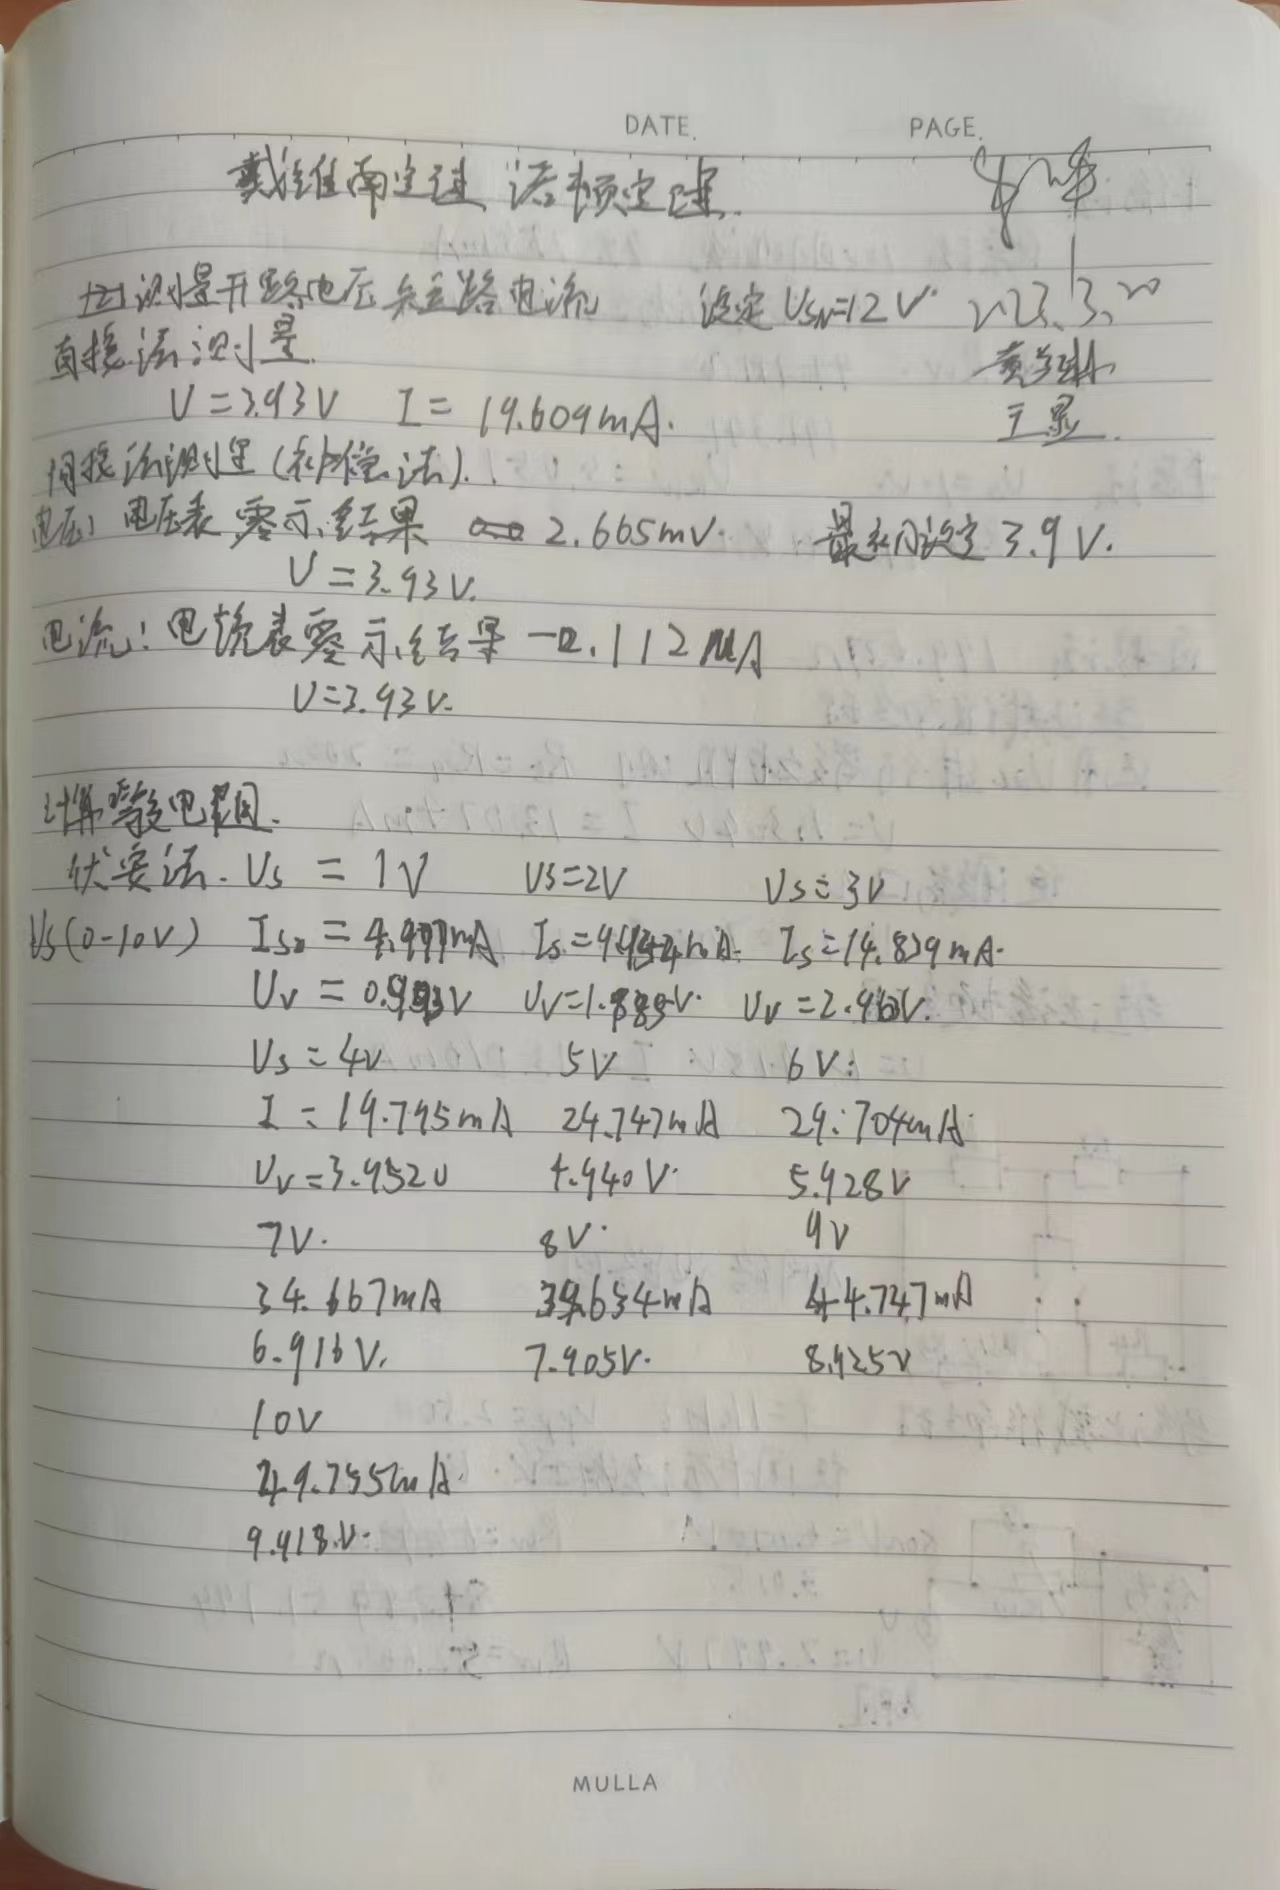
\includegraphics[width=0.4\linewidth]{数据1.jpg}
			\caption{原始数据}
		\end{minipage}
		\hfill
		\begin{minipage}[b]{0.45\linewidth}
			\centering
			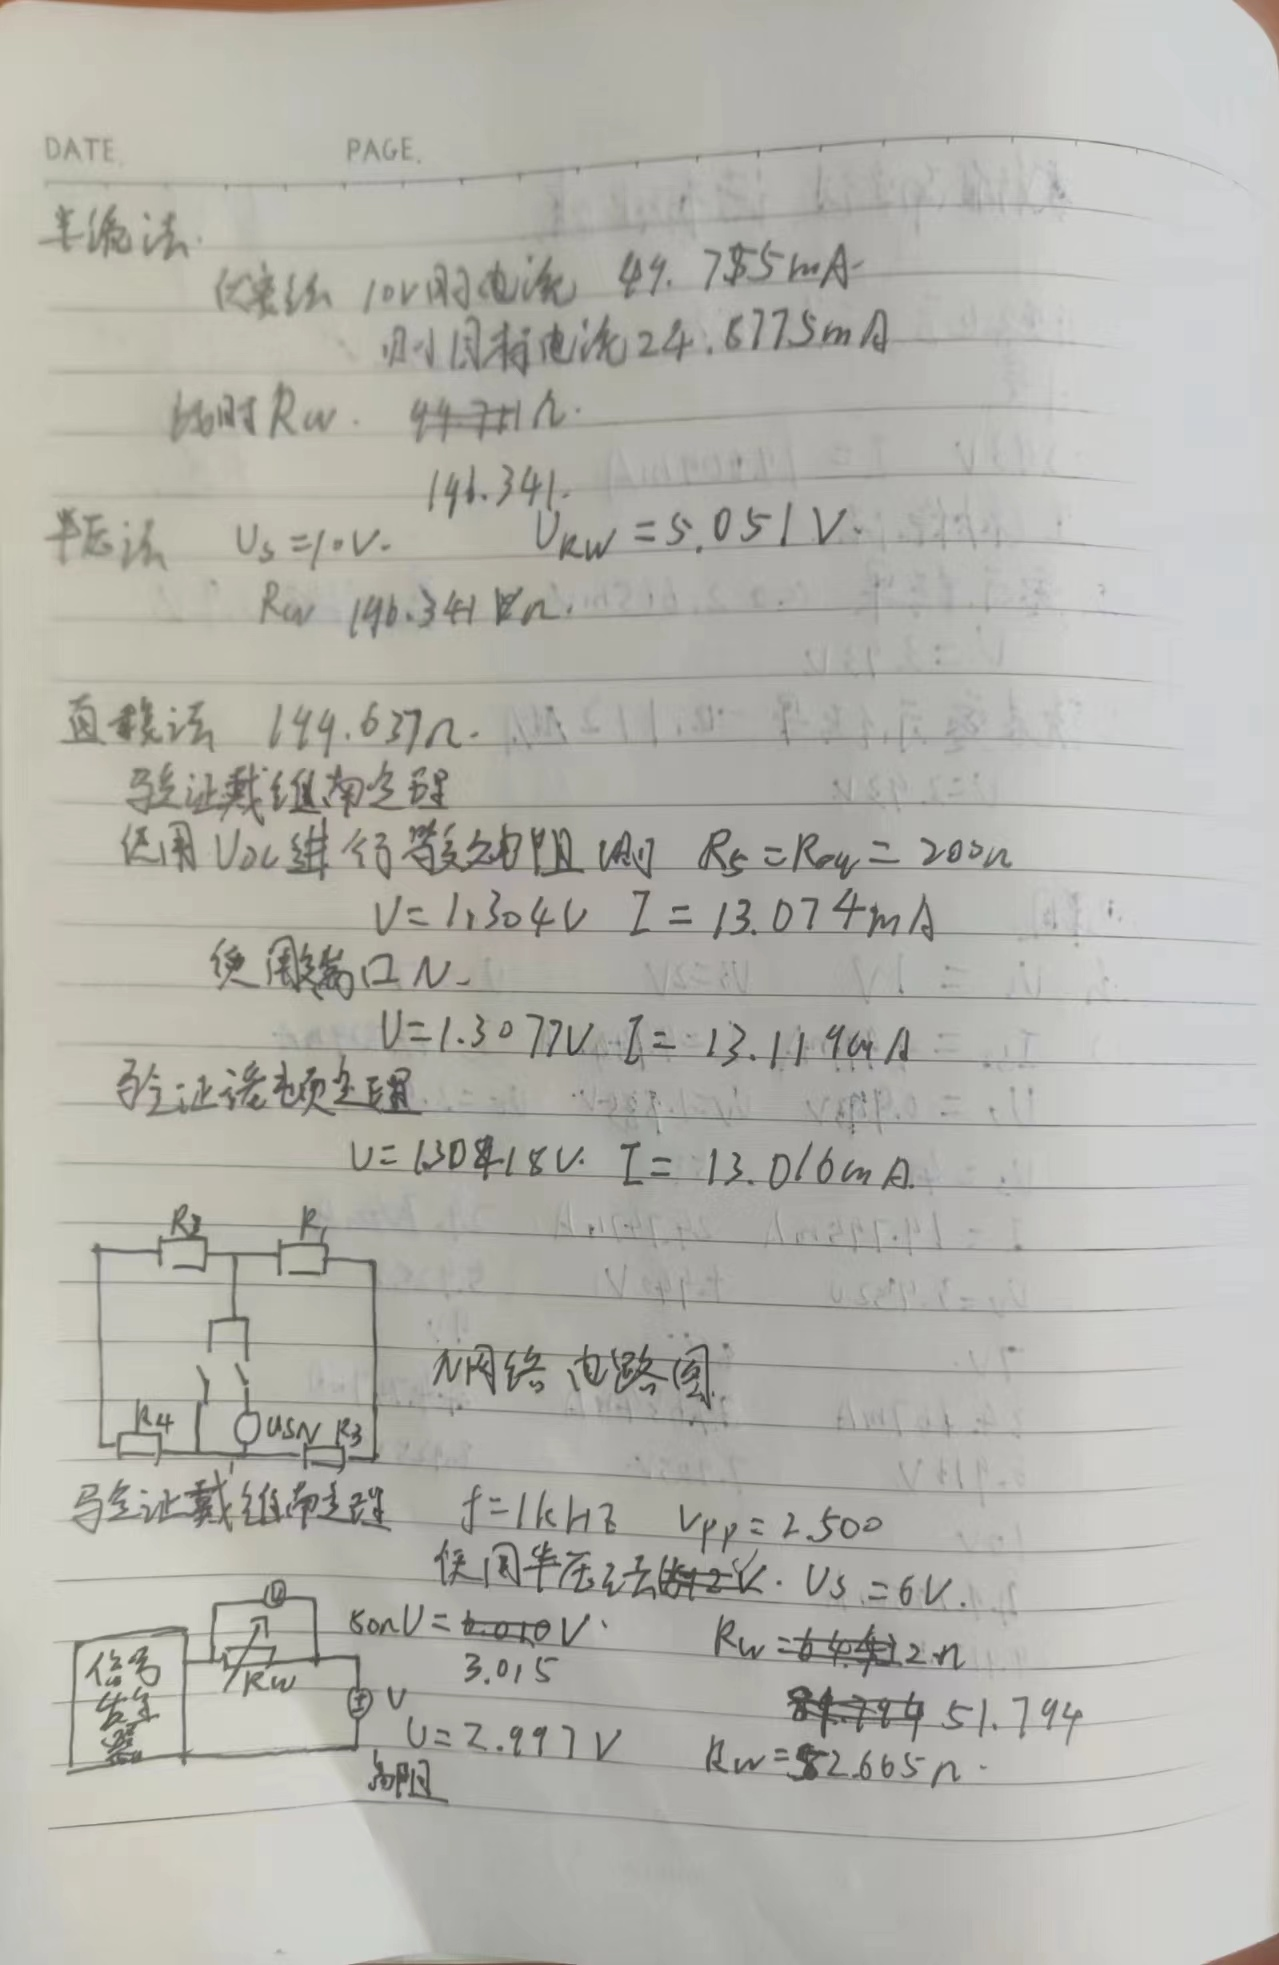
\includegraphics[width=0.4\linewidth]{数据2.jpg}
			\caption{原始数据}
		\end{minipage}
	\end{figure}
	
	\begin{figure}[H]
		\begin{minipage}[b]{0.45\linewidth}
			\centering
			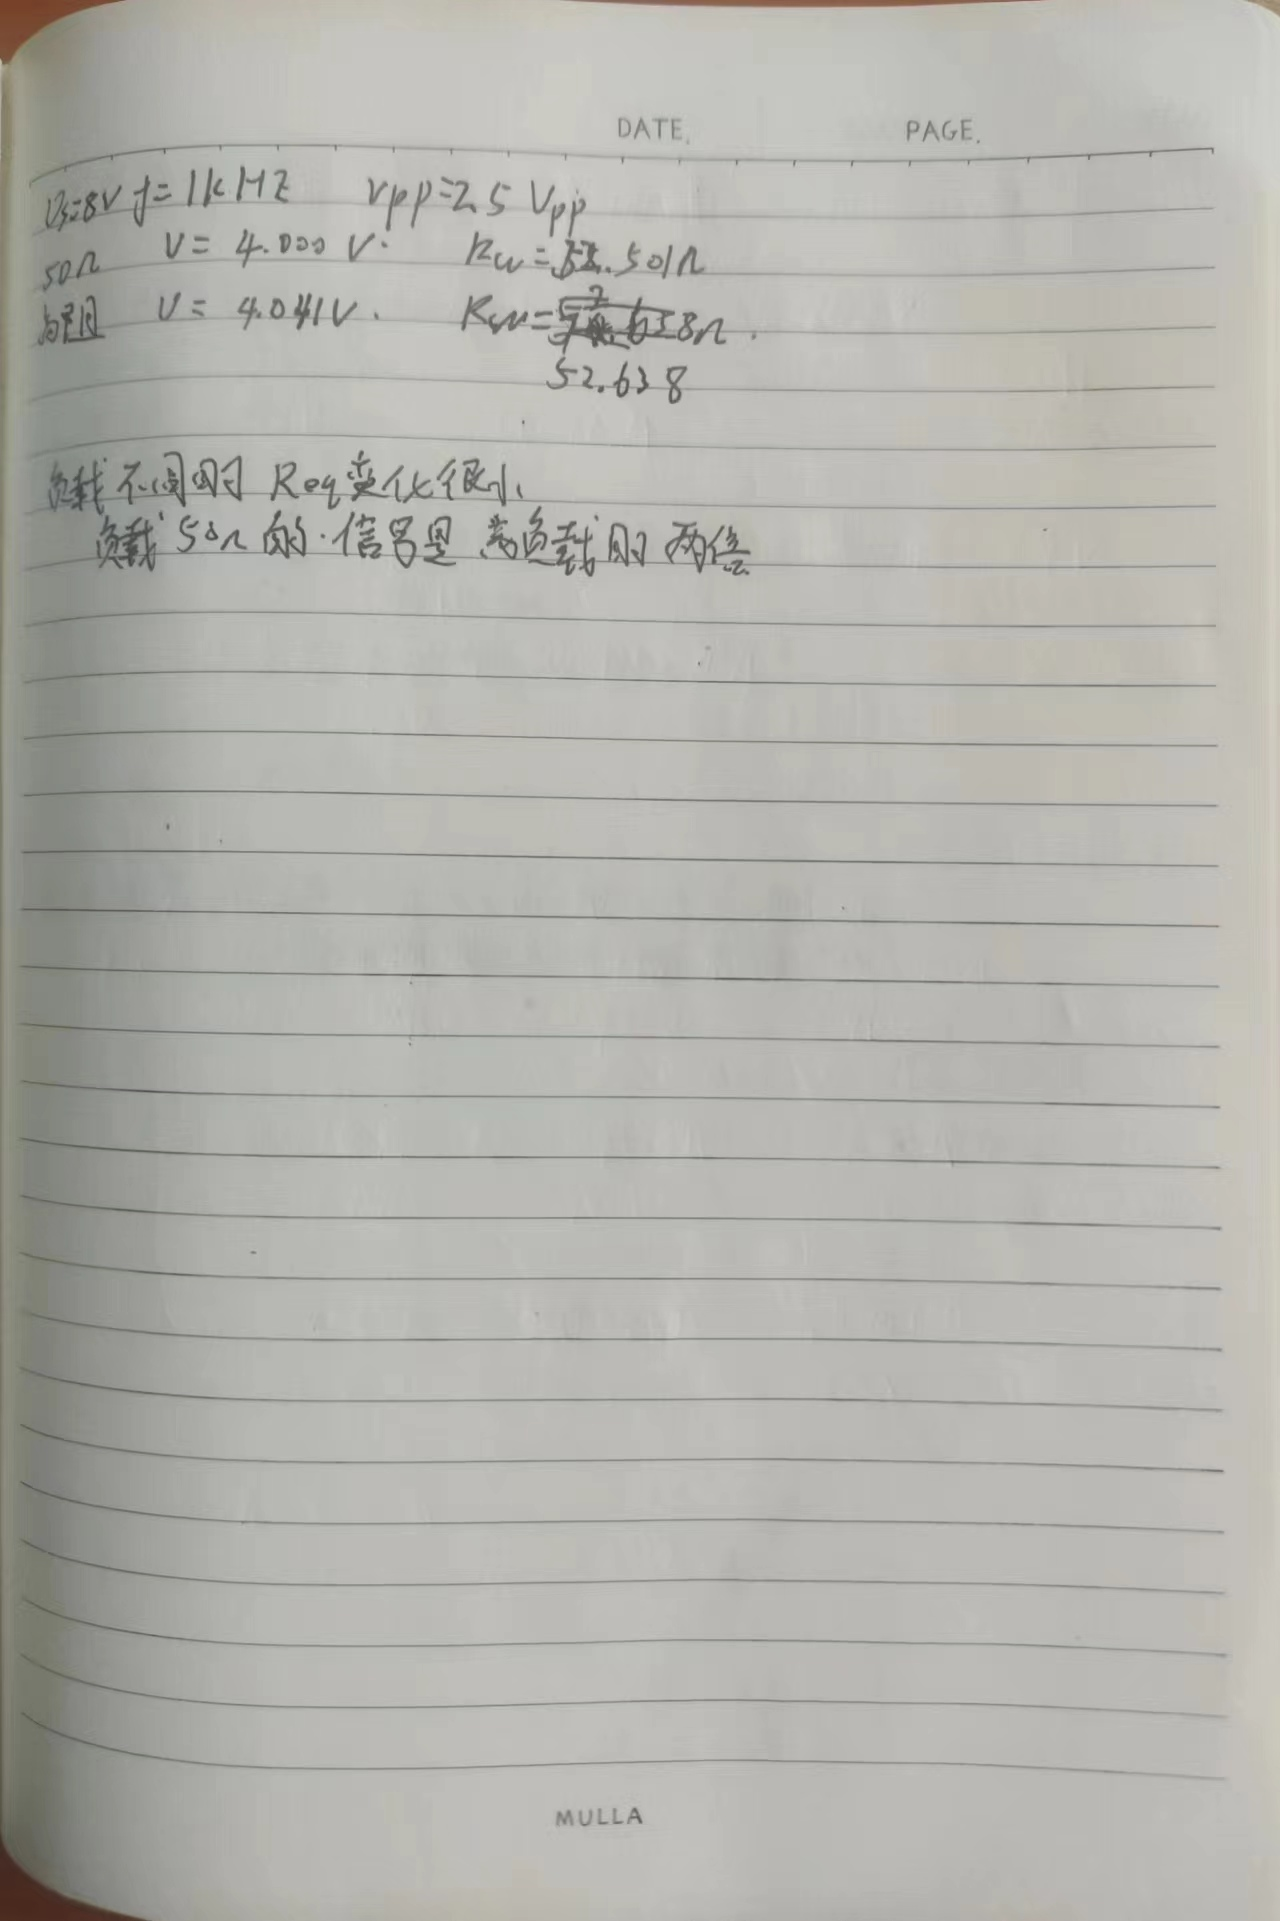
\includegraphics[width=0.4\linewidth]{数据3.jpg}
			\caption{原始数据}
		\end{minipage}
		\hfill
		\begin{minipage}[b]{0.45\linewidth}
			\centering
			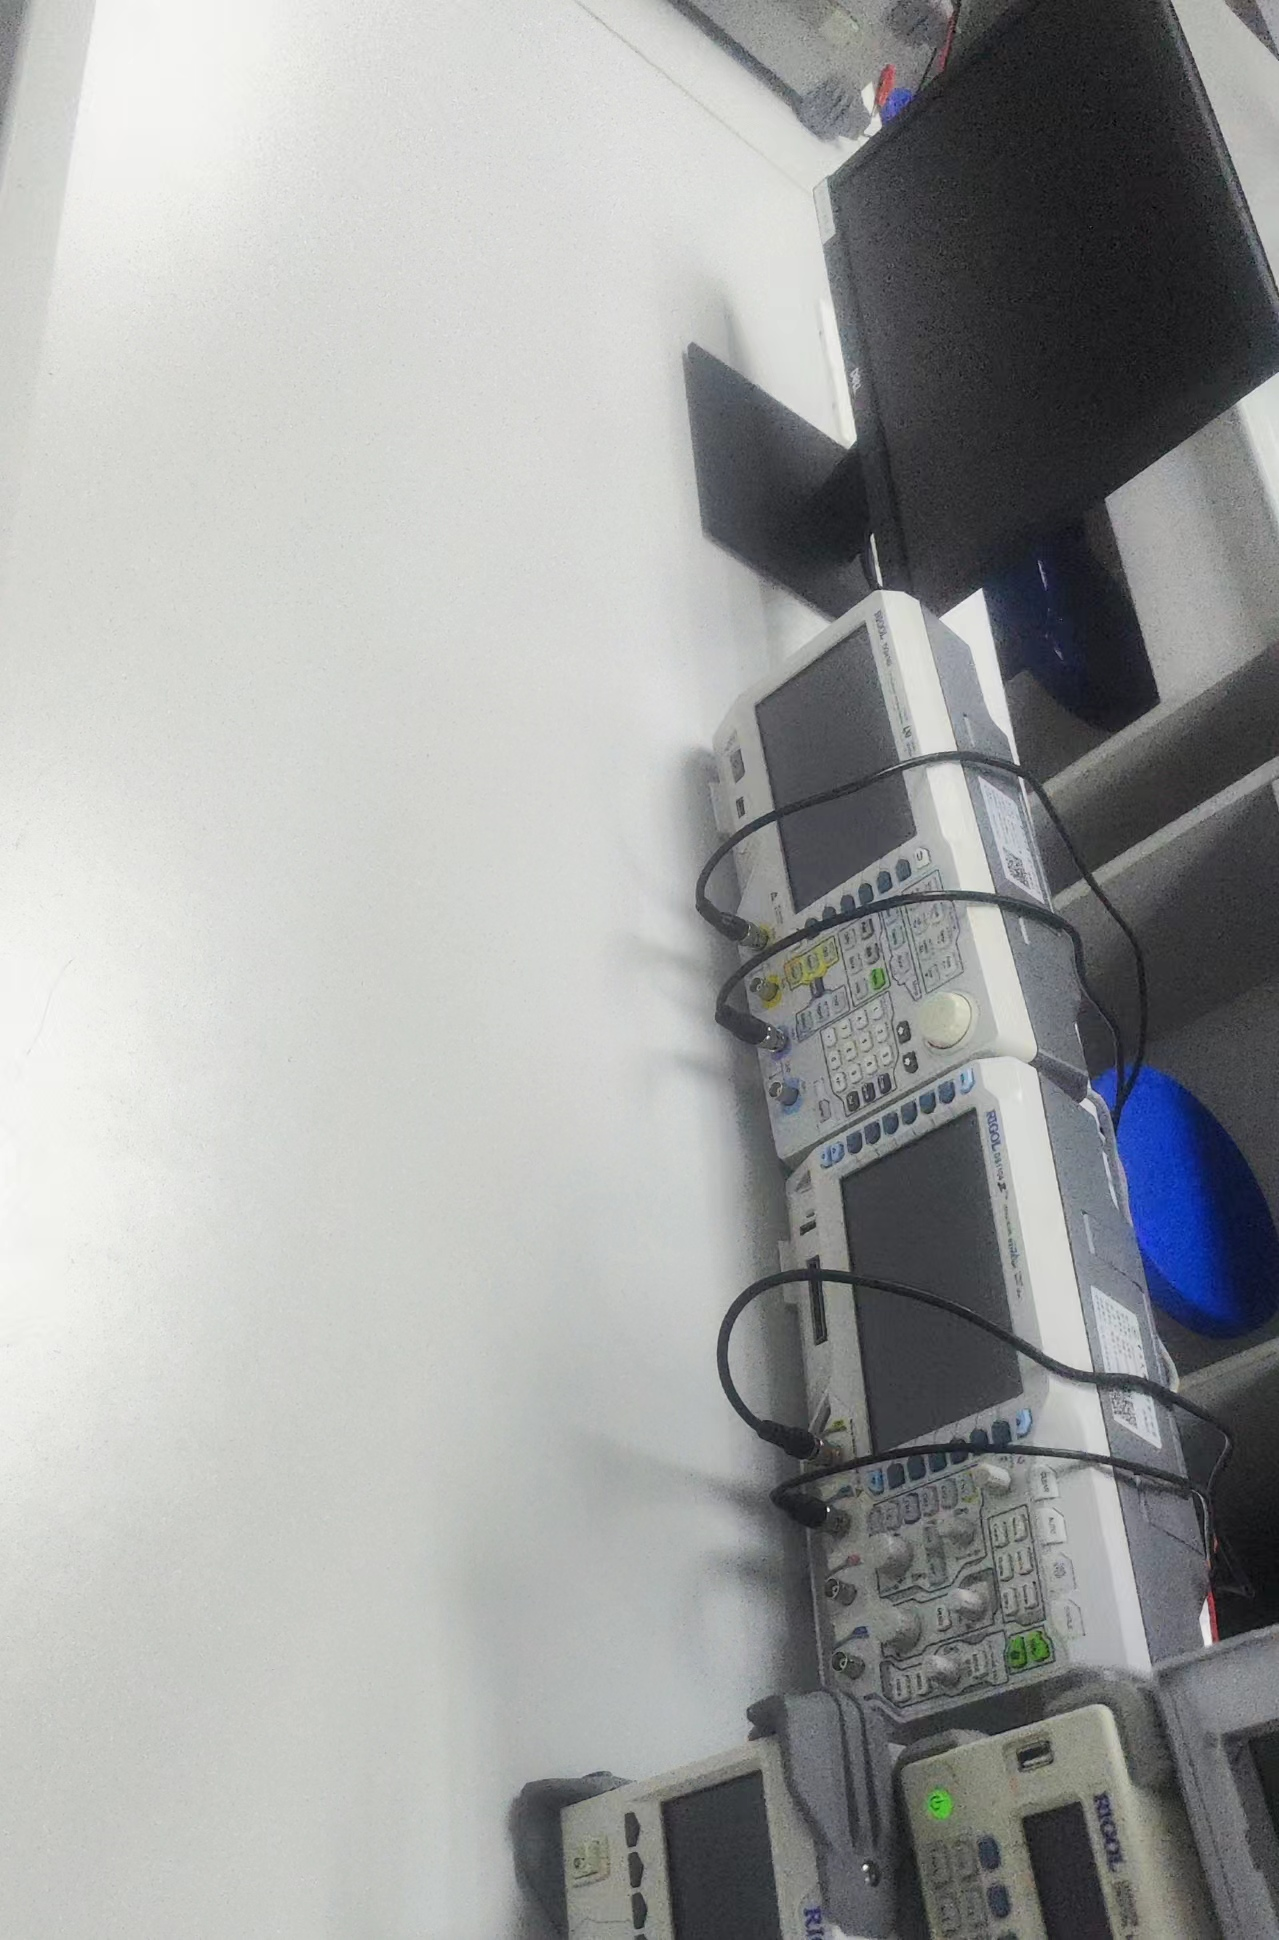
\includegraphics[width=0.4\linewidth]{桌面.jpg}
			\caption{实验桌面整理}
		\end{minipage}
	\end{figure}
	
	
	

	% ---
	
	
\end{document}